%\chapter{Contiki - a Lightweight and Flexible Operating System for Tiny Networked Sensors}
%\chapter{無線センサネットワークにおけるProtothreadsを用いたリアルタイムスケジューラ}
\chapter{問題提起}
\begin{large}
\begin{quote}
本章では,最初に,本研究が提案するT-Ringという公衆センサデータ管理システムにおける,時間概念の扱いと,それに伴った保存アルゴリズムの概念説明を行う.次に,集中管理とSynapseとのデータ管理の時間的密度と計算コストの比較を行う.詳細な設計については次章で解説する.

\end{quote}
\end{large}
\clearpage

\section{Protothreads}
既に述べたように,イベント駆動型は組み込みシステムやセンサネットワークにおいて,
主流なオペレーティングシステムとなっている.
しかし,イベント駆動型はメモリのオーバヘッド低く維持できる一方で,
ユーザが一連の処理を細かい処理に分割しなければならないため,
プログラムが書き辛いという問題が発生する(Listing\ref{lst:non-protothreads}).
%TinyOSの例
Protothreads\cite{Dunkels:2006:PSE:1182807.1182811}は
イベント駆動型プログラムをマルチスレッド型のように
記述することができるため(Listing\ref{lst:using-protothreads}),
メモリのオーバヘッドを抑えつつ,
イベント駆動型の欠点を補うことが可能となる.
本節では,Protothreadsの機能について詳しく述べる.



\begin{lstlisting}[caption=Protothredsを使用せずに記述した場合, label={lst:non-protothreads}]
struct pt {
    unsigned short lc;
};


char example(struct pt *pt) { 
    char PT_YIELD_FLAG = 1;

    if(PT_YIELD_FLAG) { ; }

    switch((pt)->lc) {
        case 0:
            while(1) { 
                do {
                    (pt)->lc = __LINE__;

        case: __LINE__:
                        if( !(condition) ) { // counter != 1000
                            return PT_WAITING;
                        } 
                } while(0);

                printf("Threshold reached\n");
                counter = 0;
            } 
    }
    PT_YIELD_FLAG = 0;
    (pt)->lc = 0;

    return PT_ENDED;
}
\end{lstlisting}



\begin{lstlisting}[caption=Protothredsを使用した場合, label={lst:using-protothreads}]
#include"pt.h"


PT_THREAD(example(structpt*pt)){
    PT_BEGIN(pt);

    while(1) {
        PT_WAIT_UNTIL(pt, counter == 1000);
        printf("Threshold reached\n");
        counter = 0;
    }
    
    PT_END(pt); 
}
\end{lstlisting}




\subsection{メモリ}
マルチスレッド型のオペレーティングシステムでは,
図\ref{fig:threads_stack}のようにそれぞれのスレッドにそれぞれのスタックを必要とする.
しかし,メモリが制限されているセンサネットワークのようなシステムでは,
スタック用のメモリは静的に保持されなければならないため,
このメモリを他の目的で使用することはできない.
\begin{figure}[htbp]
 \begin{center}
  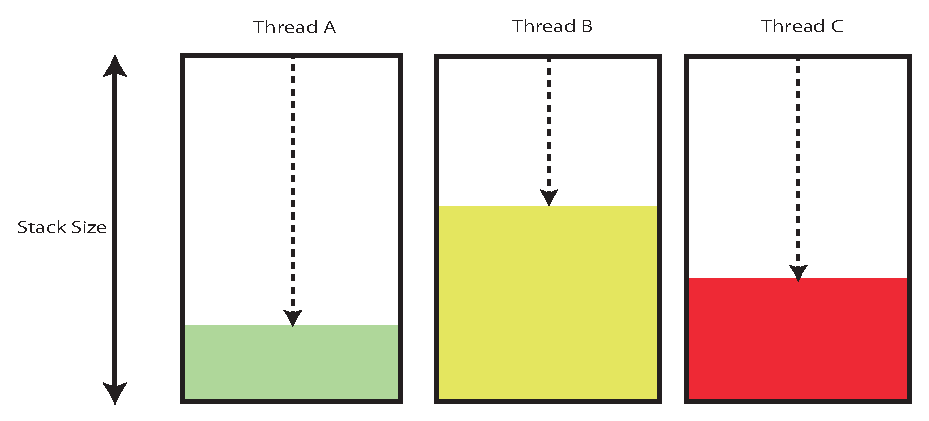
\includegraphics[width=110mm]{./images/threads_stack.eps}
 \end{center}
 \caption{一般的なスレッドモデルにおけるスタック}
 \label{fig:threads_stack}
\end{figure}

それに対して,Protothreadsにおけるスタックを図\ref{fig:protothreads_stack}に示す.
Protothreadsを使用した場合,
すべてのプログラムは同じスタックを共有し,
実行されることとなる.
つまり,Protothreadsを利用しているオペレーティングシステムではそのような事態を防ぐために,
マルチスレッドを実現しつつも,ひとつのスタックをあたかも複数個あるように見せかけている.
\begin{figure}[htbp]
 \begin{center}
  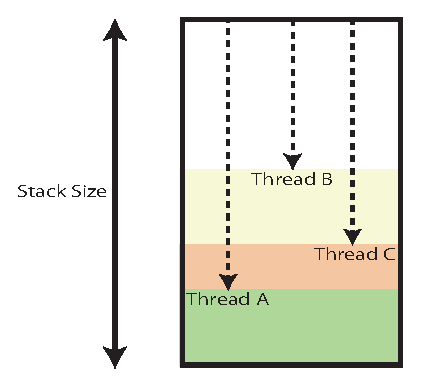
\includegraphics[width=45mm]{./images/protothreads_stack.eps}
 \end{center}
 \caption{Protothreadsにおけるスタック}
 \label{fig:protothreads_stack}
\end{figure}


\subsection{タスクの切り替え}
一般的なマルチスレッド型のオペレーティングシステムは,
タスクの割り込みがあった際には,
レジスタの状態を保存することで変数の値を保持し,
割り込まれたタスクの実行が終了したときに,
再びレジスタから変数を読み込み,
処理を途中から再開する.

しかし,Protothreadsを使用した場合,
状態をレジスタに保存することはせずに,
戻り値を利用することでタスクのCPUの利用を放棄する.
さらに,アプリケーション内の変数は静的な変数を採用しているため,
低オーバヘッドを実現しつつ,一貫性を保っている.

戻り値をもとにしたタスクの切り替えを行う際には,
スケジューラに対してプログラムのファイルの行数をreturnし,
各タスクがCPU利用権限を再度取得したとき,
行数を条件分岐し,前回中断した箇所から実行を
再開することとなる(Listing\ref{lst:using-protothreads}).

ただし,現在実行中のタスクよりも優先度の高いタスクが実行待ちになった際に,
他のマルチスレッドのオペレーティングシステムで実現されているように,
ループ内の処理を実行しているタスクに割り込みをし,
タスクを切り替えて実行することはできない.

現在では,タイマー割り込みを目的とした利用をされていない.
タイマーと現在時刻を比較し,
発火時刻を過ぎている場合,タスクを実行待ちのキューへと加える.
タイマーを実行するタスクは他のタスクと同じ優先度で周期的に実行される.




\subsection{イベント}
イベントモデルであるContikiでは,イベントを受け取るとプロセスが実行される.
ここではContikiで扱われる非同期イベント、同期イベント、ポーリングの違いについて説明する.

\subsubsection{非同期イベント}

\vspace{0.5em}非同期イベントの概念図を図\ref{fig:asynchronous_event}に示す。
非同期イベントが発生すると,
そのイベントはカーネルのイベントキューに挿入され,
後ほどイベントとして受け取られる。
%実行時にFirst In First Outで呼び出される.
%非同期イベントはポストされた後、
非同期イベントはポストされてから受諾されるまでの間、
Contikiカーネル内のイベントキューに保持される。
%Asynchronous events are delivered to the receiving process some time after they have been posted.
%Between their posting and their delivery, 
%the asynchronous events are held on an event queue inside the Contiki kernel.
イベントキュー内のイベントはカーネルによってイベント受信プロセスに送られ、
カーネルはイベントキュー内を確認し、
イベントを呼び出しているプロセスへとイベントを届ける。
%カーネルはイベント発生によってイベントをイベントキューまで運び、
%イベントキューをまとめる。
%The events on the event queue are delivered to the receiving process by the kernel.
%The kernel loops through the event queue and 
%delivers the events to the processes on the queue by invoking the processes.

非同期イベントの受信プロセスはある特定のプロセスである場合と、
すべての実行中のプロセスである場合がある。
イベントの受信者がある特定のプロセスだった場合、
カーネルはイベントを届けるためにこのプロセスを呼び出す。
イベントの受信者がシステム内のすべてのプロセスだった場合、
カーネルは同じイベントをすべてのプロセスへと順次届けていく。
%The receiver of an asynchronous event can either be a specific process, or all running processes.
%When the receiver is a specific process, the kernel invokes this process to deliver the event.
%When the receiver of an event is set to be all processes in the system,
%the kernel sequentially delivers the same event to all processes, 
%one after another.

非同期イベントはprocess\_post関数によってポストされる.
process\_post関数ははじめにキュー内にイベントのためのメモリ空間があるかどうかを確認するために,
現在のイベントキューのサイズを調べる.
もしメモリに空きがなければエラーを返し,
メモリに空きがあった際にはイベントをキューの最後に挿入する.

%Asynchronous events are posted with the process\_post() function. The internals of the process\_post() function is simple.
%It first checks the size of the current event queue to determine if there is room for the event on the queue.
%If not, the function returns an error.
%If there is room for the event on the queue,
%the function inserts the event at the end of the event queue and returns.

\begin{figure}[htbp]
 \begin{center}
  \includegraphics[width=115mm]{./images/fifo.eps}
 \end{center}
 \caption{非同期イベントの実行}
 \label{fig:asynchronous_event}
\end{figure}




\subsubsection{同期イベント}

\vspace{0.5em}図\ref{fig:synchronous_event}は同期イベントにおける概念図である。
非同期イベントに対して,
同期イベントはポストされたとき,
即座にイベントとして受諾される。
%When a synchronous event is posted,
%the event is immediately delivered to the receiving process.
同期イベントはある特定のプロセスにのみポストされる点も非同期イベントとは異なっている。
%Unlike asynchronous events, 
%synchronous events are delivered directly when they are posted.
%Synchronous events can only be posted to a specific processes.

同期イベントは即座に実行されるため,
同期イベントがポストされることは関数を呼び出すことに等しい.
%Because synchronous events are delivered immediately,
%posting a synchronous event is functionally equivalent to a function call: 
すなわち、イベントを届けられたプロセスは直接よびだされ、
イベントをポストしたプロセスは受信プロセスによるイベントの処理が終了するまで
他の処理を行うことはできない。
%the process to which the event is delivered is directly invoked, 
%and the process that posted the event is blocked until the receiving process has finished processing the event.
しかしながら、受信プロセスはイベントが同期的にポストされたか、非同期的にポストされたかを知らされない。
%The receiving process is, however, not informed whether the event was posted synchronously or asynchronously.

\begin{figure}[htbp]
 \begin{center}
  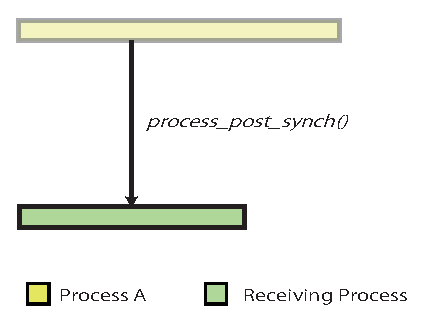
\includegraphics[width=40mm]{./images/synchronous_event.eps}
 \end{center}
 \caption{同期イベントの実行}
 \label{fig:synchronous_event}
\end{figure}


\subsubsection{ポーリング}

\vspace{0.5em}ポーリングリクエストはその他のイベントと異なる
ポールされたプロセスはprocess\_poll()関数によって呼び出され,
この関数がプロセス上で呼び出されるとそのプロセスは可能な限り早急にスケジューリングされる.

A poll request is a special type of event. A process is polled by calling the function process\_poll().
Calling this function on a process causes the process to be scheduled as quickly as possible.
The process is passed a special event that informs the process that it has been polled.

ポーリングはインタラプトからプロセスを実行する手法であり,
process\_poll()関数はプリエンプティブモードから安全に呼び出されるプロセスモジュールにおける,
唯一の関数である.

%Polling is the way to make a process run from an interrupt.
%The process\_poll() function is the only function in the process module that is safe to call from preemptive mode.

%\section{イベントタイマー}
%Contikiオペレーティングシステムには



\section{既存システムにおける問題意識}
イベント駆動モデルではタスクの中断をしないことを前提に設計されているため,
現在のセンサネットワーク用のオペレーティングシステムでは省資源性かつ低オーバヘッドであることと,
リアルタイム性のサポートはトレードオフの関係にある.
しかし,ターゲットトラッキングなどの状況においては,
通常時は省資源性かつ低オーバヘッドを実現し,
イベントが生じた際にはリアルタイム処理を行うことが必要となってくる.
それにも関わらず,現在双方を両立可能としたセンサネットワーク用のオペレーティングシステムは存在していない.

また,Protothreadsが
%イベント駆動型のオペレーティングシステムに実装されていながら,
マルチスレッド型のオペレーティングシステムとの親和性があると推測できることは既に述べたが,
既存のProtothreadsの実装ではイベントに優先度をつけることなく,
First In First Out(FIFO)の要領でイベントを呼び出している(図\ref{fig:asynchronous_event}).
本研究では環境モニタリングやターゲットトラッキングを想定環境としているため,
イベントの到着順でスケジューリングすることは好ましくない.
例えば,優先度の高いタスクが到着したときに既に多量のタスクが実行待ち状態となっている場合に,
高優先度のタスクが実行される頃には,既にそのタスクに実行する価値はない可能性がある.
したがって,既存手法とは別のアルゴリズムを用いてスケジューリングする必要がある.


%前述のとおり,一般的なマルチスレッド型のオペレーティングシステムでは,
%スレッド切り替え時にレジスタの状態を保存するのに対して,

Protothreadsでは,現在実行中のタスクよりも優先度の高いタスクが実行待ちになった際に,
他のマルチスレッドのオペレーティングシステムで実現されているように,
ループ内の処理を実行しているタスクに割り込みをし,
タスクを切り替えて実行することはできない.
これはタスクがreturnを発行するまでスケジューラが実行されないためである.


\section{本研究のアプローチ}


\section{まとめ}
本章では,まず,保存ピアの計算量を削減し,Synapseよりもデータ管理の時間的密度が高いアルゴリズムを提案することを述べた.次に,T-Ringにおいて時間という属性をDHTにおける保存ピアの決定における一つ要素としてではなく,保存ピアの変更を行うための要素として扱うことを述べた.そして,時間的密度,計算コストの観点から集中管理,Synapse,T-Ringの3つの手法の比較を行った.また,センサデータの時間的特殊性に着目した多次元センサデータ分散管理システムであるT-Ringの詳細な設計概念,設計実装について述べた.T-RingはP2Pのトポロジとして,代表的なアルゴリズムであるChordに準拠した1Dトーラスを用いている.保存ピアの参加や離脱なども同様にChordに準拠している.また,多次元データを扱うにあたり,Z-orderにより1次元化に言及した.時間的特殊性については,chunkとSPという2つの時間概念を導入し,保存ピア変更の基準とした.また,ユーザがT-Ringシステムを用いて,データ取得のクエリを送る際の,形式を定義した.



